\documentclass{article}
\usepackage[utf8]{inputenc}
\usepackage[margin=1in]{geometry}
\usepackage{enumitem}
\usepackage{amsmath}
\usepackage{listings}
\usepackage{color}
\usepackage{booktabs}
\usepackage[font=small, labelfont=bf]{caption}
\usepackage[T1]{fontenc}

% macro to select a scaled-down version of Bera Mono (for instance)
\makeatletter
\newcommand\BeraMonottfamily{%
  \def\fvm@Scale{0.85}% scales the font down
  \fontfamily{fvm}\selectfont% selects the Bera Mono font
}
\makeatother

\definecolor{codegreen}{rgb}{0,0.6,0}
\definecolor{codegray}{rgb}{0.5,0.5,0.5}
\definecolor{codepurple}{rgb}{0.58,0,0.82}
\definecolor{backcolour}{rgb}{0.95,0.95,0.92}

\lstdefinestyle{mystyle}{
    backgroundcolor=\color{backcolour},
    commentstyle=\color{codegreen},
    keywordstyle=\color{magenta},
    numberstyle=\tiny\color{codegray},
    stringstyle=\color{codepurple},
    basicstyle=\BeraMonottfamily\footnotesize,
    breakatwhitespace=false,         
    breaklines=true,                 
    captionpos=b,                    
    keepspaces=true,                 
    numbers=left,                    
    numbersep=5pt,                  
    showspaces=false,                
    showstringspaces=false,
    showtabs=false,                  
    tabsize=2
}
\lstset{style=mystyle,
        otherkeywords={True,False}
}

\title{CS249 Fall 2020\\
       Problem Set 2: Statistical Inference II}
\author{Christopher Munoz Cortes}
\date{\today}

\usepackage{natbib}
\usepackage{graphicx}

\begin{document}

\maketitle

\section{Hypothesis Testing}
Assume a friend of yours currently has a salary of \$70k per year. She is
considering a switch in her career, and has narrowed down her choices to
three different options. She has been able to find the following data points
for entry-level salaries (in thousand dollars) for these three choices:
\begin{enumerate}
\item 143 102 119 157 146 61 119 85 87 102
\item 77 143 108 76 92 87 145 60 86 27
\item 19 83 87 55 115 41 71 66 101 99
\end{enumerate}
Assume that these data points are IID observations, and the difference between 
them can only be attributed to noise. Additionally, assume that after
a career change your friend’s salary will be a sample from the same distribution 
as the one behind your observed data points.
\begin{enumerate}[label={(\alph*)}]
    \item Can your friend expect an increase in her salary on average if she
    chooses \#1?
    
    An appropriate null hypothesis to answer this question would be the following
    one-tail test: $H_0: \mu_0 \leq 70$. If we can reject $H_0$, then we can assert
    that the population mean is higher than \$70k, and conclude that our friend
    should expect, on average, an increase in her salary. 
    Since $\frac{p}{2} = 0.0009 < \alpha = 0.05$
    and $t>0$ we reject $H_0$. As a consequence, our friend should expect an
    increase in her salary on average if she chooses \#1.
    
    \item Is there any difference between the average salary of the three 
    choices?
    
    Here we define $H_0: \mu_1 = \mu_2 = \mu_3$ as our null hypothesis and use an 
    ANOVA test to verify it. The result of the test shows that we have enough evidence
    to reject the null hypothesis, since $p = 0.04 < \alpha = 0.05$. As a
    consequence, we assert that there is a difference between the average salary of
    the three choices.
    
    \item Is there any difference between the average salary of \#1 and \#3?
    
    We can answer this question testing the following null hypothesis: $H_0: \mu_1
    = \mu_3$ and verifying its validity. Since $p = 0.01 < \alpha = 0.05$ we reject 
    $H_0$ and assert that the mean salary for choice 1 and choice 2 are different.
\end{enumerate}

\begin{lstlisting}[language=Python, caption=Code for Question 1 \emph{Hypothesis
Testing}]
import numpy as np
from scipy import stats

y_1 = np.array([143, 102, 119, 157, 146, 61, 119, 85, 87, 102])
y_2 = np.array([77, 143, 108, 76, 92, 87, 145, 60, 86, 27])
y_3 = np.array([19, 83, 87, 55, 115, 41, 71, 66, 101, 99])

# Part (a): H_0: mean >= 70k
mu_0 = 70
t_stat, p_val = stats.ttest_1samp(y_1, mu_0)
print(f"t-stat: {t_stat}")
print(f"p-value: {p_val/2}")

# Part (b): H_0: mu_1 = mu_2 = mu_3
f_stat, p_val = stats.f_oneway(y_1, y_2, y_3)
print(f"f-stat: {f_stat}")
print(f"p-value: {p_val}")

# Part (c): H_0: mu_1 = mu_3
t_stat, p_val = stats.ttest_ind(y_1, y_3, equal_var=True)
print(f"t-stat: {t_stat}")
print(f"p-value: {p_val}")
\end{lstlisting}

\pagebreak

\section{Regression to the Mean}
\begin{enumerate}[label={(\alph*)}]
    \item Assume $x$ represents the height of the father and $y$ 
    represents the height of the son. Standardize the two 
    covariates. You can use the following code:
    
    \lstinline{x = (x - np.mean(x)) / np.std(x)}
    
    \lstinline{y = (y - np.mean(y)) / np.std(y)}
    
    Plot \lstinline{y} vs. \lstinline{x} in a scatter plot in Python.
    \begin{figure}[h]
        \centering
        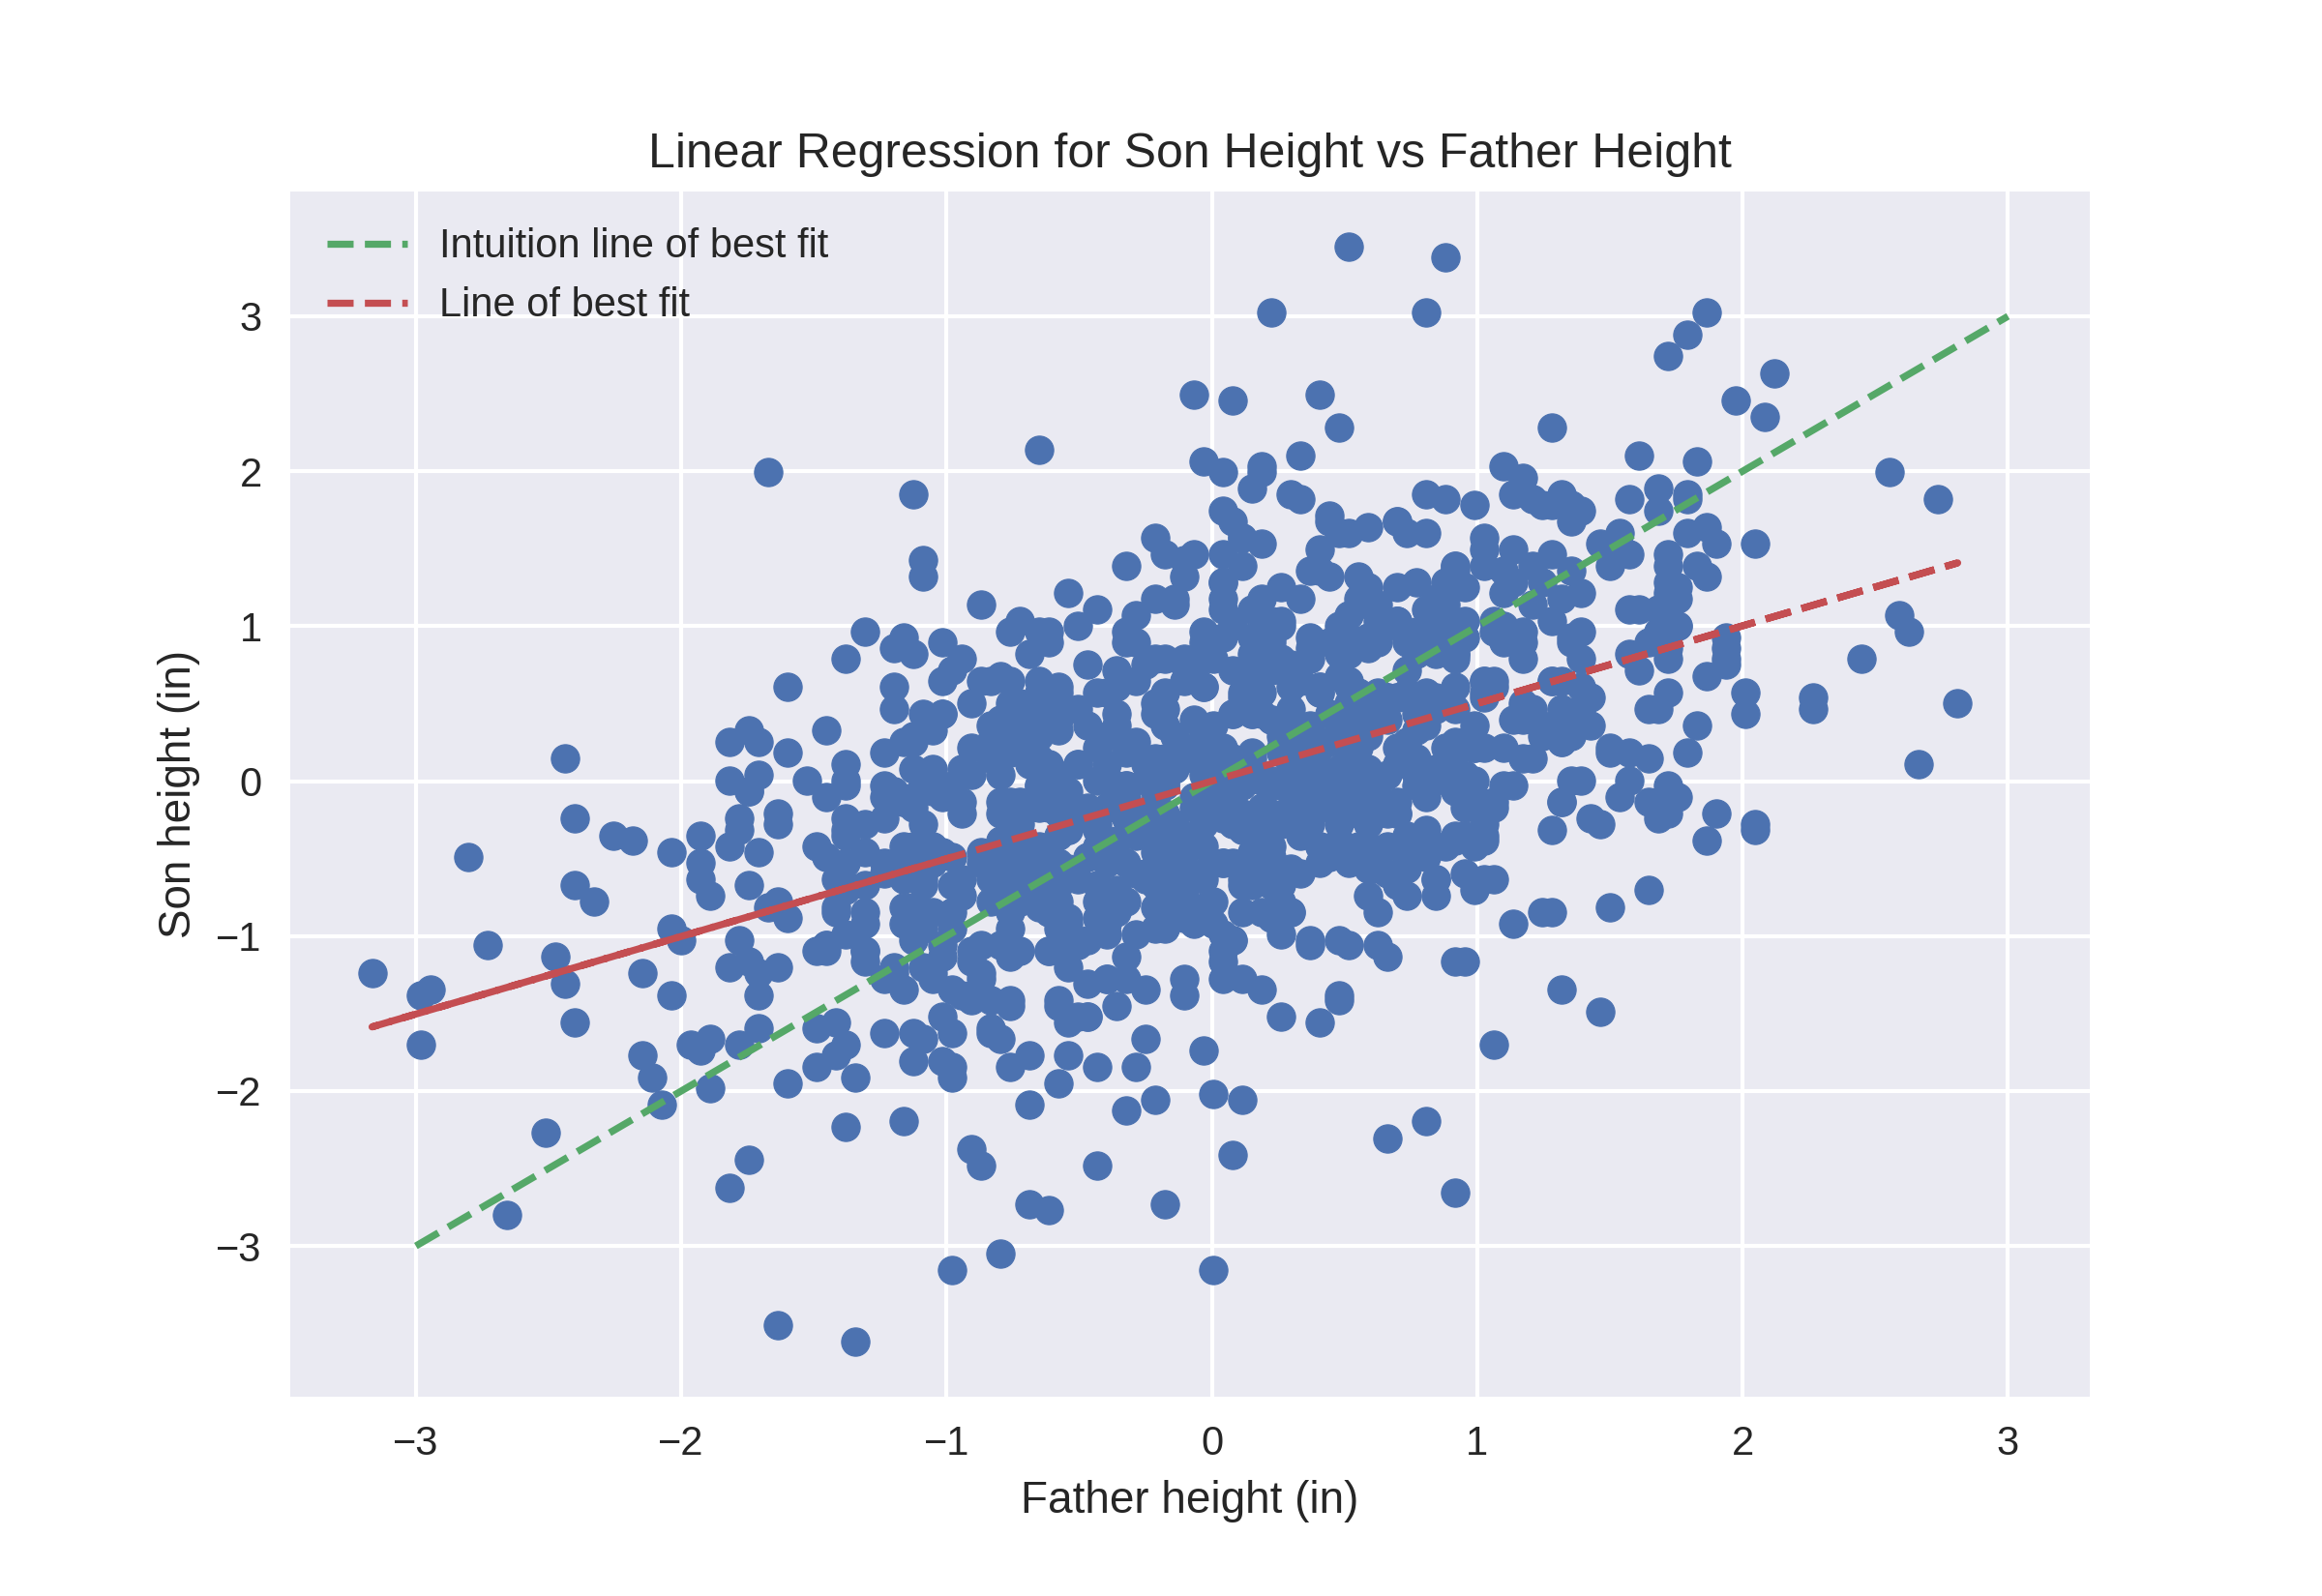
\includegraphics[scale=0.7]{scatter_father_son_height.png}
        \caption{\lstinline{y} vs. \lstinline{x}}
        \label{fig:father_son}
    \end{figure}
    
    \item Based on your intuition and without fitting a model, draw the line corresponding to the linear regression for this data.
    
    See Figure \ref{fig:father_son}.
    
    \item Fit a linear regression in Python where the response variable is 
    \lstinline{y}. Draw the line corresponding to the fitted linear regression in the
    scatter plot. Does this line match your intuition from the previous part?
    
    The line corresponding to the fitter linear regression does not match the line I
    plotted based on my intuition. See Figure \ref{fig:father_son} above.
    %TODO: add equation for the line of best fit
    
    \item Based on the fitted regression line, if a father is 10 inches taller than
    the average, how much greater is the expected height of the son compared to the
    average? And if a father is 10 inches shorter than the average, how much smaller
    is the expected height of the son compared to the average?
    
    If a father is 10 inches taller than the average, the expected height of the son
    is 5.14 inches taller than the average. Conversely, if a father is 10 inches
    shorter than average, the expected height of the son is 5.14 inches shorter
    than average.
    
    \item Based on the answer to the previous part, do you think it is fair to say
    that heights become more and more ``average'' over time? Read about ``regression 
    to the mean'' and revisit your answer.
    
    If we didn't take the regression error into consideration, the results from the
    previous part would lead us to believe that the heights do become more ``average''
    over generations. However, this is a naive interpretation that ignores the fact
    that the actual $y_i$ values will not be exactly where the model predicts them to 
    be. Some of them will be closer to the mean, while other will be further from it.
    In other words, we when take the error in the regression predicting $y$ from $x$,
    this interpretation is incorrect.
    
    \begin{lstlisting}[language=Python, caption=Standard Error and Confidence
    Interval for $T$]
import pandas as pd
from google.colab import drive
import matplotlib.pyplot as plt
from sklearn.linear_model import LinearRegression

# Mount drive
drive.mount('/content/drive')
df = pd.read_csv('/content/drive/My Drive/father_son.txt', delim_whitespace=True)

# Standardize the two covariates
def standardize_feature(feature):
  return (feature - np.mean(feature)) / np.std(feature)

x = standardize_feature(df['Father'])
y = standardize_feature(df['Son'])

# Part (a): plot y vs. x
fig, ax = plt.subplots()
ax.scatter(x, y)

# Part (b): plot intuition line of best fit (y=x)
x_int = np.linspace(-3,3)
y_int = x_int
ax.plot(x_int, y_int, linestyle='dashed', color='C1')

# Part (c): fit a linear regression
x = x.values.reshape(-1, 1)
y = y.values.reshape(-1,1)
model = LinearRegression()
model.fit(x,y)
y_hat = model.predict(x)
ax.plot(x, y_hat, linestyle='dashed', color='C2')
ax.legend(['Intuition line of best fit', 'Line of best fit'])

# Part (d)
# Father 10 in taller than the average
x_father = df['Father'].mean() + 10

# Transform the value to match the scale of the model fit
x_father = (x_father - df['Father'].mean()) / df['Father'].std()
x_father = np.array([x_father])

# Son height for x_father
y_hat_son = model.predict(x_father.reshape(-1,1))
y_hat_son = y_hat_son[0][0] * df['Son'].std() + df['Son'].mean()
print(f"The son is {y_hat_son - df['Son'].mean()} inches taller than the average")

# Part (e)
# What if the father is 10 in shorter than the average?
x_father_2 = df['Father'].mean() - 10
x_father_2 = (x_father_2 - df['Father'].mean()) / df['Father'].std()
x_father_2 = np.array([x_father_2]).reshape(-1,1)

y_hat_son_2 = model.predict(x_father_2)
y_hat_son_2 = y_hat_son_2[0][0] * df['Son'].std() + df['Son'].mean()
print(f"The son is {np.abs(y_hat_son_2 - df['Son'].mean())} inches shorter than the average")
\end{lstlisting}
\end{enumerate}
\pagebreak

\section{Linear Regression}
In this problem, we are going to see what happens if we use a linear regression to 
model the relationship between two independent random variables.
\begin{enumerate}[label={(\alph*)}]
    \item Simulate 1000 data points from a normal distribution with mean 0 and standard
    deviation 1. Assign it to a variable named $x$. Simulate another 1000 data points
    from a similar normal distribution and assign them to variable $y$. Run a linear
    regression of $y$ vs. $x$. Use \texttt{statsmodels} to view the statistical
    properties of the model. What is the slope of the model? Report your observations.
    
    I generated $y$ drawing samples from a normal distribution $N(0,1)$. The linear regression results from fitting $y$ vs. $x$ with \texttt{statsmodels} are shown below:
    \begin{figure}[h]
        \centering
        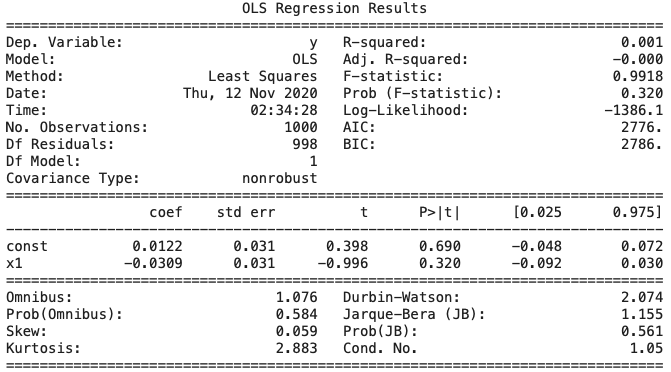
\includegraphics[scale=0.5]{ols_res.png}
        \caption{OLS Regression Results with \texttt{statsmodels}.}
        \label{fig:ols_res}
    \end{figure}
    
    As shown in Figure \ref{fig:ols_res}, the slope of the fitted line is -0.0309.
    
    \item Repeat the simulation in the previous part 100 times and gather the
    slopes in a list. Draw the distribution, and report your conclusions based
    on the result.
    \begin{figure}[h]
        \centering
        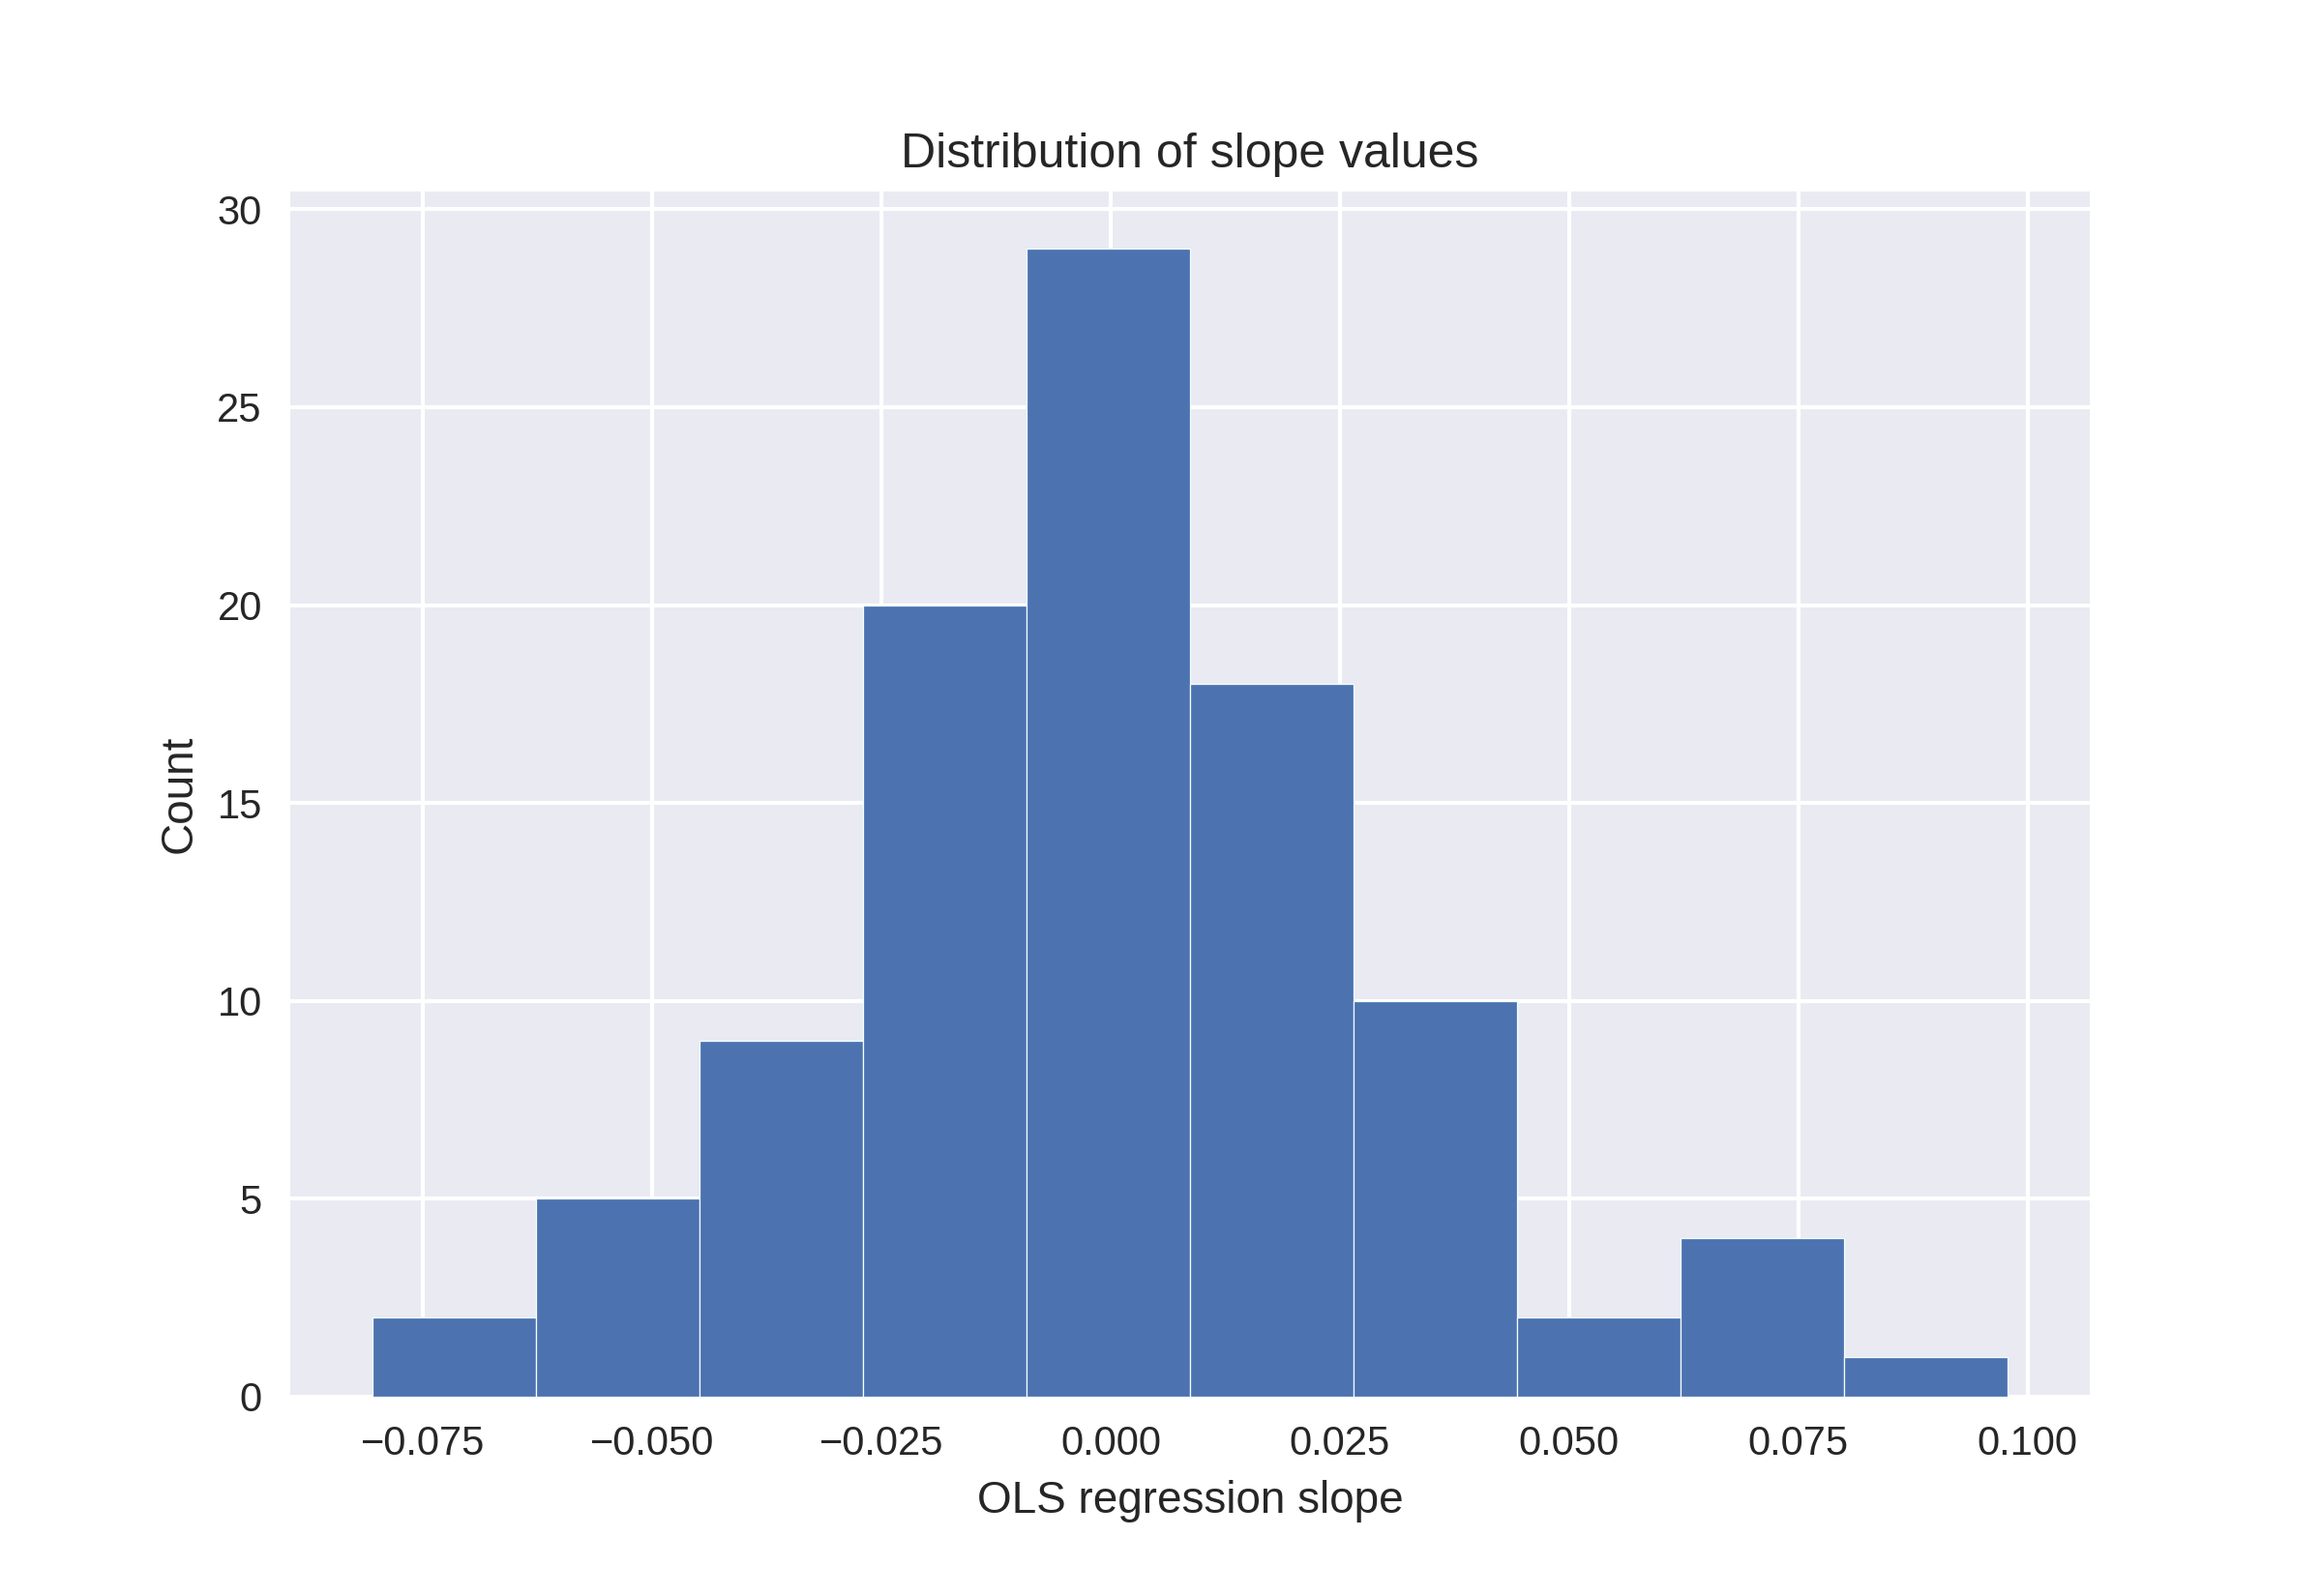
\includegraphics[scale=0.5]{slopes_dist.png}
        \caption{Distribution of slope values}
        \label{fig:slopes}
    \end{figure}
    
    The distribution for the slope values is centered around ~0 and has a standard
    deviation of 0.03. The slope reported by the linear regression model is roughly 
    within one standard deviation of the distribution of the slope values found by 
    running several simulations.
\begin{lstlisting}[language=Python, caption=Standard Error and Confidence]
import numpy as np
import statsmodels.api as sm
import numpy as np
import matplotlib.pyplot as plt

np.random.seed(0)

# Simulate 1000 data points from a normal distribution with a mean 0 and std 1
x = np.random.normal(0,1,1000)
y = np.random.normal(0,1,1000)

# Fit the model
x_with_intercept = sm.add_constant(x)
model = sm.OLS(y, x_with_intercept).fit()
y_hat = model.predict(x_with_intercept)

# Print the results
print(model.summary())

# Repeat the simulation 100 times
slopes = []
for i in range(100):
  x = np.random.normal(0,1,1000)
  y = np.random.normal(0,1,1000)
  x_with_intercept = sm.add_constant(x)
  model = sm.OLS(y, x_with_intercept).fit()
  slopes.append(model.params[1])

# Get the mean and std dev of the distribution
slope_std = np.std(slopes)
slope_mean = np.mean(slopes)
print(f"Slope std: {slope_std}")
print(f"Slope mean: {slope_mean}")

# Plot the distribution
plt.hist(slopes, ec='azure')
plt.title('Distribution of slope values')
plt.xlabel('OLS regression slope')
plt.ylabel('Count')
plt.savefig('/content/drive/My Drive/slopes_dist.png', dpi=300)
\end{lstlisting}
    
\end{enumerate}
\pagebreak

\section{Linear Regression Properties}
\begin{enumerate}[label={(\alph*)}]
    \item Assume we have fitted a linear regression model with an intercept to our 
    data. Prove that the sum of residuals in the fitted model is equal to zero:
    \[
        \sum_{i=0}^n \hat{\varepsilon_i} = 0
    \]
    Proof:
    \begin{align*}
        \sum_{i=0}^n \hat{\varepsilon_i} &= 
        \sum_{i=0}^n (Y_i - \widehat{Y_i}) \\
        &= Y - X(X^TX)^{-1}X^TY \\
        &= Y - X X^{-1} (X^T)^{-1}  X^T Y \\
        &= Y - I I Y \\
        &= Y - Y = 0
    \end{align*}
    
    \item We can write the equation for a linear regression model fitted to a dataset 
    with $p$ features and $n$ data points as
    \[
        Y_i = \hat{\beta}_0 + \sum_{j=1}^p \hat{\beta}_j X_{i,j} + \hat{\varepsilon_i}
    \]
    where $X_{i,j}$ is the value of $j$-th feature for $i$-th data point and $Y_i$ is
    the response variable for the $i$-th data point. Assume we have 
    \emph{centered features} in our data, meaning
    \[
        \dfrac{1}{n} \sum_{i=1}^n X_{i,j} = 0
    \]
    prove that the value of the intercept in the fitted model is equal to the
    average of the response variable in our data:
    \[
        \hat{\beta_0} = \dfrac{1}{n} \sum_{i=1}^n Y_i
    \]
    Proof:
    \begin{align*}
        \hat{\beta_0} &= \dfrac{1}{n} \sum_{i=1}^n Y_i \\
        &= \dfrac{1}{n} \sum_{i=1}^n (\hat{\beta_0} + \sum_{j=1}^p \hat{\beta_j}
        X_{i,j} + \hat{\varepsilon_i}) \\
        &= \dfrac{1}{n} \left(n\hat{\beta_0} + \sum_{i=1}^n \sum_{j=1}^p \hat{\beta_j}
        X_{i,j} + \sum_{i=1}^n\hat{\varepsilon_i} \right) \\
        &= \hat{\beta_0} + \sum_{j=1}^p \hat{\beta_j} \left(\dfrac{1}{n}
        \sum_{i=1}^n X_{i,j}\right) \\
        &= \hat{\beta_0}
    \end{align*}
\end{enumerate}

%\bibliographystyle{plain}
%\bibliography{references}
\end{document}
